\chapter{Projekt}
\section{Wprowadzenie}
Aplikacja została przygotowana na potrzeby przedmiotu \textit{''Podstawy Sztucznej Inteligencji''}. Do jej wykonania wykorzystano repozytorium \textbf{ArztSamuel/Applying\_EANNs}\cite{aeann_psi}. Zadanie polegało na zastosowaniu biblioteki Pytorch\cite{NEURIPS2019_9015}, dla języka Python. Należało połączyć skrypt, napisany w języku Python do obliczania aktualnej zmiany pozycji dla pojazdu znajdującego się na mapie, za pomocą \textbf{Jednokierunkowej Sieci Neuronowej}(ang. \textit{Feedforward Neural Network (FNN)}), wraz z aplikacją Unity napisanej w języku C$\#$; Dodatkowo należało dołączyć ten skrypt do algorytmu genetycznego (\textbf{GA}). Połączenie GA i FNN służy do wytrenowania pojazdów autonomicznych, których celem jest przejechanie utworzonej trasy.  

\subsection{Feedforward Neural Network}
Jest to typ sieci neuronowej, która jest jednokierunkowa (od wejścia, do wyjścia). W takich sieciach nie ma możliwości przepływ informacji w drugą stronę.\cite{lnn}

\begin{figure}[H]
    \includegraphics[width=\textwidth]{images/fnn.pdf}
    \caption{Schemat sieci neuronowej FNN}
    \label{fig:fnn}
\end{figure}

\subsection{Algorytm genetyczny}
Zdaniem algorytmu genetycznego jest znalezienie optymalnego rozwiązania w skończonej liczbie iteracji, bądź obejmującego minimalny optymalny wynik dopasowania. Algorytm polega na losowym utworzeniu populacji możliwych wyników, a następnie próbie ich dopasowania. Najlepsze wyniki są wybierane, i przy zastosowanym w kodzie \textbf{wybieraniu elitarnym} zachowywane do następnej populacji. Następnie występuje krzyżowanie oraz mutacja wyników. Celem tych dwóch operacji jest wyłonienie potencjalnych najlepszych rezultatów. Po operacji mutowania wybierane są najlepsze rozwiązania z możliwym uwzględnieniem ''elitarnych'' wyników z pierwszej selekcji. Operacje się powtarza aż do znalezienia optymalnego rozwiązania, bądź przejściu maksymalnej ilości iteracji. Na końcu zwracany jest najlepszy osobnik z ostatniej populacji.

\begin{figure}[H]
    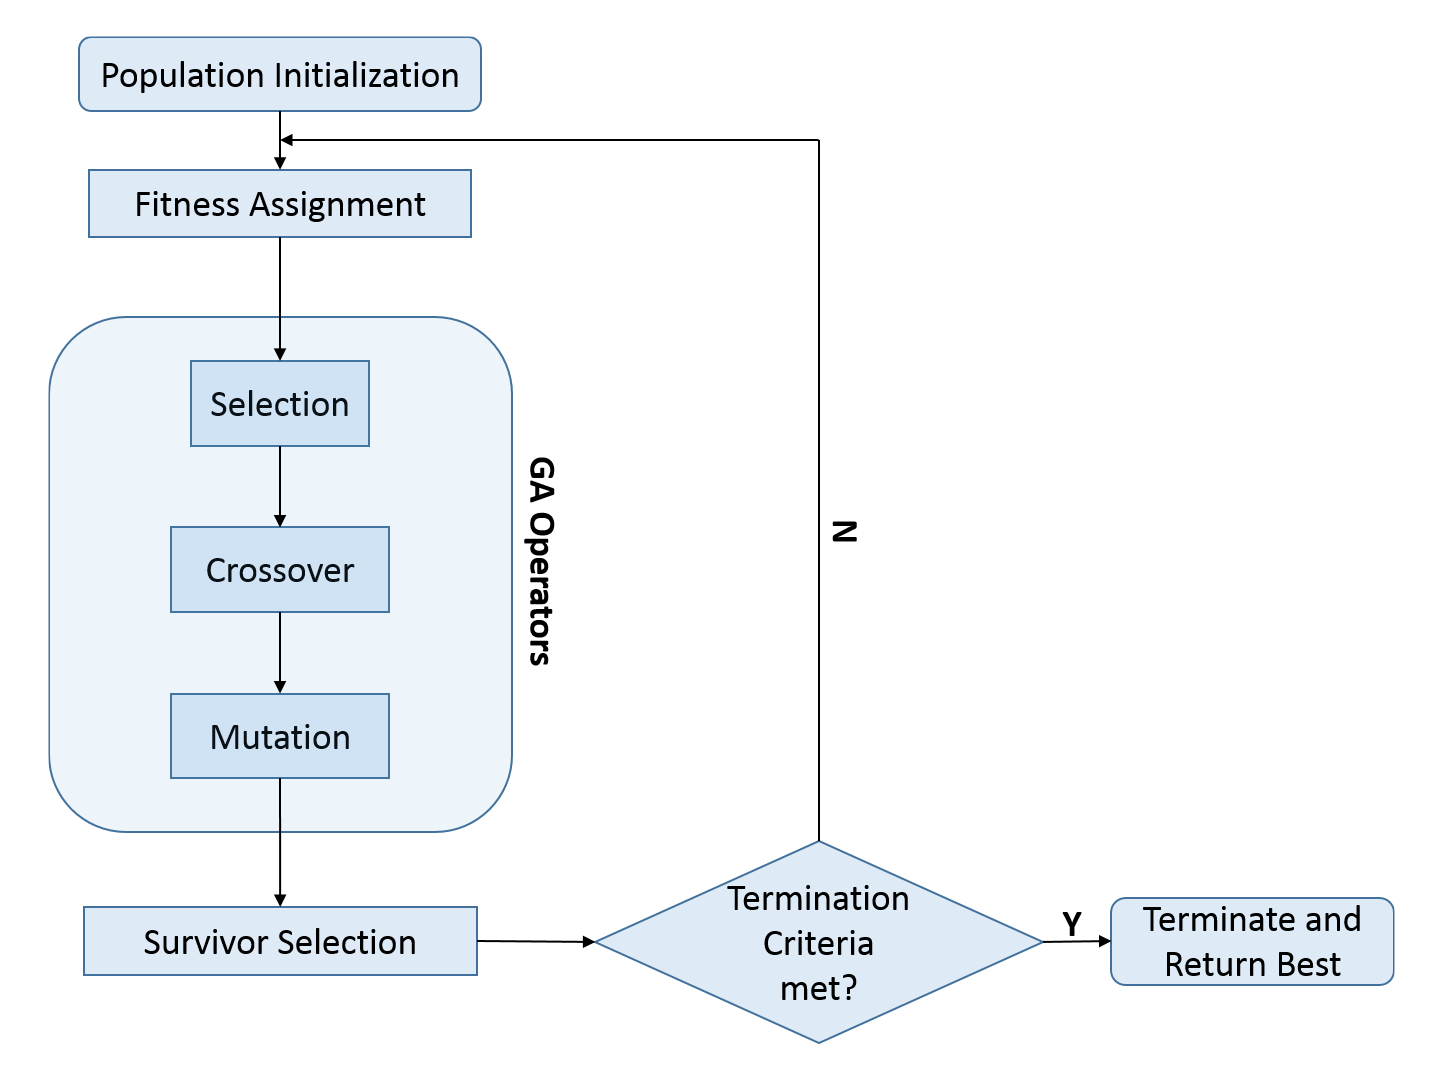
\includegraphics[width=\textwidth]{images/ga_schema.png}
    \label{fig:ga}
    \caption{Schemat algorytmu genetycznego\cite{ai}}
\end{figure}
\clearpage

\subsection{Algorytmy obsługujące żądania z Unity}
Poniżej przedstawiono dwa algorytmy, które są wykorzystywane we współpracy z Unity, do obliczeń. Aby uruchomić proces należy wykorzystać język python w wersji 3

\begin{lstlisting}[language=sh, caption={Wywłanie programu}]
$ python3.8 main_2,py <sciezka_do_pliku_wag> <ilosc_wejsc>
\end{lstlisting}

program po wczytaniu pliku i zapisaniu go do zmiennej, przechodzi w tryb oczekiwania na wejściu standardowym. W celu obsłużenia programu należy skorzystać z jednej z dwóch możliwości: \textbf{0}, \textbf{1 <dane na wejsciu>} (\textit{np: 1 1 2 3 4 5}). Podanie \textbf{0} kończy program, zaś wykorzystanie \textbf{1}, bądź dowolnego innego znaku odczyta wszystko co znajduje się za pierwszym znakiem. W tym przykładzie ''\textit{1 1 2 3 4 5}'', są to liczby ''\textit{1 2 3 4 5}''. Liczby te następnie są przekazywane do metody \textbf{calc}, znajdującej się w klasie \textbf{net}. Metoda ta oblicza dane za pomocą wag oraz sieci FNN dane występujące na wyjściach. Następnie dane zwrócone przez metodę są zapisywane na wyjściu standardowym. Po tym kroku program przechodzi w tryb oczekiwania.
\clearpage
\lstinputlisting[language=Python, caption={Algorytm służący do obsługi żądania z terminala}, label=frag:main_py]{main_2.py}
\clearpage
\lstinputlisting[language=Python, caption={Algorytm sieci neuronowych działający dla podanych wag, wejść oraz ilości wyjść}, label=frag:net_py]{net.py}
\ \\
Poniżej przedstawiono algorytm w formie schematu blokowego:
\begin{figure}[H]
    \includegraphics[width=\textwidth]{images/main_2.py.pdf}
    \caption{Schemat blokowy algorytmu w pliku main\_2.py}
    \label{fig:schemat}
\end{figure}